\subsection{Explain the origin of the molecular potential within the Born-Oppenheim approximation and discuss the vibrational and rotational structure of diatomic molecules.}


\ldots

\begin{figure}[!h]
    \centering
    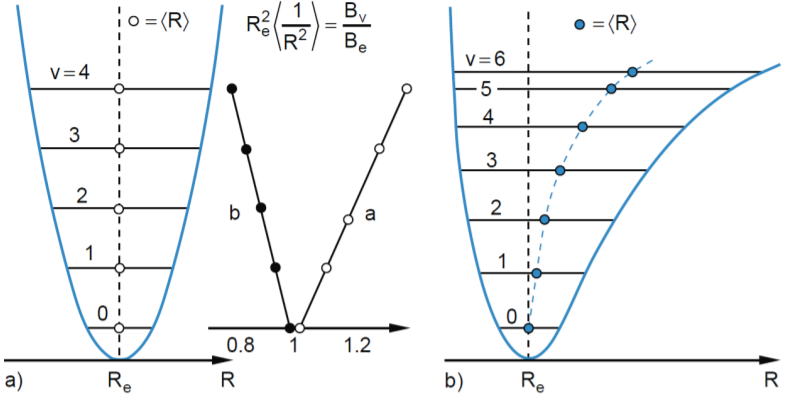
\includegraphics[width=.8\textwidth]{Q20/images/AfstandMellemEnerginiveauerneIToForskelligePotentialleApproksimationer.PNG}
    \caption{}
    \label{fig:Q20_AfstandMellemEnerginiveauer}
\end{figure}

\begin{figure}[!h]
    \centering
    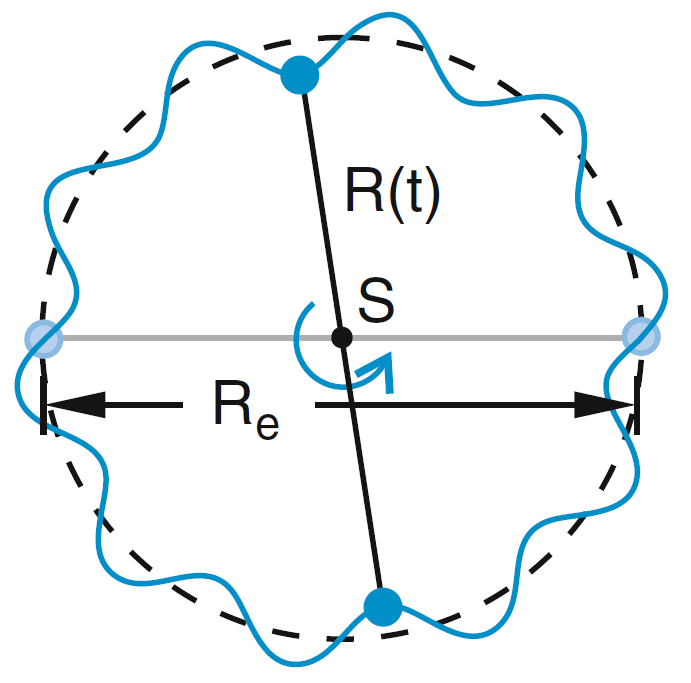
\includegraphics[width=.35\textwidth]{Q20/images/VibratingRotor.PNG}
    \caption{}
    \label{fig:Q20_VibratingRotor}
\end{figure}

\begin{figure}[!h]
    \centering
    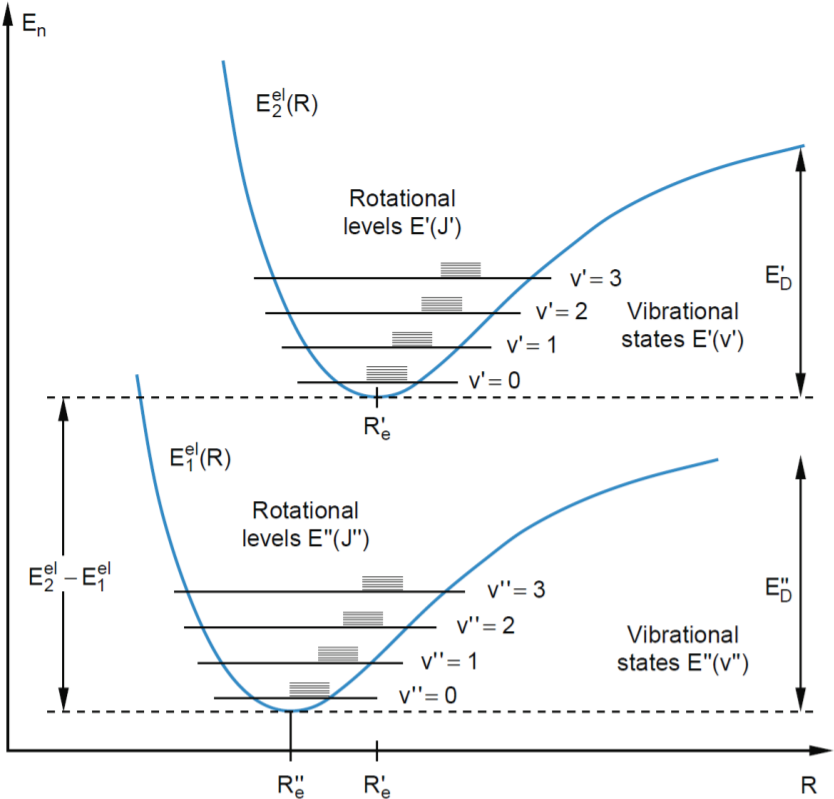
\includegraphics[width=.8\textwidth]{Q20/images/VibrationOgRotationIPotentialDiatomartMolekyle.PNG}
    \caption{}
    \label{fig:Q20_VibrationOgRotationPotential}
\end{figure}